%%%%%%%%%%%%%%%%%%%%%%%%%%%%%%%%%%%%%%%%%%%%%%%%%%%%%%%%%%%%%%%%%%%%%%%%%%%%%%%%
% TUM-Vorlage: Wissenschaftliche Arbeit
%%%%%%%%%%%%%%%%%%%%%%%%%%%%%%%%%%%%%%%%%%%%%%%%%%%%%%%%%%%%%%%%%%%%%%%%%%%%%%%%
%
% Rechteinhaber:
%     Technische Universität München
%     https://www.tum.de
% 
% Gestaltung:
%     ediundsepp Gestaltungsgesellschaft, München
%     http://www.ediundsepp.de
% 
% Technische Umsetzung:
%     eWorks GmbH, Frankfurt am Main
%     http://www.eworks.de
%
%%%%%%%%%%%%%%%%%%%%%%%%%%%%%%%%%%%%%%%%%%%%%%%%%%%%%%%%%%%%%%%%%%%%%%%%%%%%%%%%
%TOEDIT
%choose one of the following languages and comment the other. You might compile twice when changing the language
%\def\lan{deutsch}		
\def\lan{english}
%%%%%%%%%%%%%%%%%%%%%%%%%%%%%%%%%%%%%%%%%%%%%%%%%%%%%%%%%%%%%%%%%%%%%%%%%%%%%%%%
\documentclass[%
    fontsize=11pt, % Schriftgröße
    twoside=off % kein einseitiges Layout
]{scrbook} % Dokumentenklasse: KOMA-Script Book
\usepackage{scrlayer-scrpage} % Anpassbare Kopf- und Fußzeilen
%\usepackage[ansinew]{inputenc}
%\usepackage[latin1]{inputenc}
%\usepackage[applemac]{inputenc}
\usepackage[utf8]{inputenc} % Textkodierung: UTF-8
\usepackage[T1]{fontenc} % Zeichensatzkodierung

\def\deutsch{deutsch}
\def\english{english}
\ifx\lan\deutsch 
\usepackage[ngerman]{babel} % Deutsche Lokalisierung
\else
\usepackage[english]{babel} % Englische Lokalisierung
\addto\captionsenglish{\renewcommand*\contentsname{Table of Contents} }
\fi
%\usepackage[ngerman]{babel} % Deutsche Lokalisierung

% Added by peter below 
\usepackage{graphicx}

\usepackage{float} % Get support for floating figures

\usepackage{tikz}

\usetikzlibrary{arrows,decorations.pathmorphing,backgrounds,positioning,fit,matrix}

\usepackage{pgfplots}

\usepackage{lettrine}

\usepackage{tabularx}

\usepackage[export]{adjustbox}

\usepackage{subfig}

\usepackage{varioref} % More descriptive referencing

\usepackage{listings} % Code application environment

\usepackage{multicol}

\usepackage[style=numeric,sortcites=true,block=nbpar,backend=bibtex8]{biblatex} % Get support for the bibliography 

\usepackage{pdfpages}            % Inserting pdf pages


% added by peter above


\usepackage{amsmath}

\usepackage{amsthm}

\usepackage{amssymb}

\usepackage{makeidx}

\usepackage[english]{babel} %Language package

\usepackage{blindtext} %inserting random text

\usepackage{subfig} % Get support for the subfigures

\usepackage{float} % Get support for floating figures

\usepackage{mathrsfs} % Get support for mathematical symbols

\usepackage{graphicx} % Get support for LaTeX graphics

\usepackage{microtype}% Disable ligatures

\DisableLigatures[f]{encoding = *, family = * } % Get support for multiple language packages

\usepackage{mathptmx}

%\usepackage{fancyhdr} ----------------------------------------------

\usepackage{nopageno}

\usepackage{array}

\usepackage{multirow}

%\usepackage{appendix} % Get support for the appendix
\usepackage[titletoc]{appendix}

\usepackage{txfonts} % Get support for times New Roman

%\usepackage[ansinew]{inputenc} 

\usepackage{xcolor} % Get support for coloring parts of the text

\usepackage[autostyle,german=guillemets]{csquotes}

\usepackage[style=numeric,sortcites=true,block=nbpar,backend=bibtex8]{biblatex} % Get support for the bibliography 

%\usepackage[a4paper,vmargin={25mm,30mm},hmargin={30mm,20mm},footnotesep=1cm]{geometry} % Adjust the geometry of the outcome pdf

%\usepackage[a4paper,footnotesep=1cm]{geometry} % Adjust the geometry of the outcome pdf

\usepackage[T1]{fontenc}

\usepackage{lmodern} 

\usepackage{graphicx} % Required for including images
\graphicspath{{images/}} % Set the default folder for images

\usepackage{enumitem} % Required for manipulating the whitespace between and within lists

\usepackage{subfig} % Required for creating figures with multiple parts (subfigures)

\usepackage{amsmath,amssymb,amsthm} % For including math equations, theorems, symbols, etc

\usepackage{varioref} % More descriptive referencing

\usepackage[onehalfspacing]{setspace} 

\usepackage{listings} % Code application environment

\usepackage{multicol}

\usepackage[section]{placeins} % Figures and tables remain in their section

\usepackage{here} 

\usepackage[subfigure]{tocloft}
\usepackage{tocloft}

\usepackage{wrapfig}

\usepackage{notoccite}

\usepackage[ ]{titlesec}  %

\usepackage{titlesec, blindtext, color}

\usepackage{eso-pic}

\usepackage{algorithm}

\usepackage{algpseudocode}

\usepackage{etoolbox}
% --------------------------------------------------
%
%        ORIGINAL PACKAGES BELOW
%
% --------------------------------------------------




\usepackage{graphicx} % Grafiken

% Schriftart Helvetica:
\usepackage[scaled]{helvet}
\renewcommand{\familydefault}{\sfdefault}

% Silbentrennung:
\usepackage{hyphenat}
\hyphenation{TUM in-te-res-siert} % Eigene Silbentrennung
%\tolerance 2414
%\hbadness 2414
%\emergencystretch 1.5em
%\hfuzz 0.3pt
%\widowpenalty=10000     % Hurenkinder
%\clubpenalty=10000      % Schusterjungen
%\vfuzz \hfuzz

%\usepackage[hidelinks]{hyperref} % Hyperlinks
\usepackage[onehalfspacing]{setspace} % 1,5facher Zeilenabstand
\usepackage{calc} % Berechnungen
\usepackage{enumitem} % Mehr Kontrolle über itemize-, enumerate- und description-Umgebungen
\usepackage{relsize} % Schriftgröße in Abhängigkeit von aktueller anpassen
\usepackage{tabularx} % Flexiblere Tabellen
\usepackage{caption} % Anpassen von Beschriftungen

% Nummerierung von Abbildungen & Tabellen durchgängig, statt nach Kapiteln:
\usepackage{chngcntr}
\counterwithout{figure}{chapter}
\counterwithout{table}{chapter}

% Abkürzungen, Glossare:
\usepackage[%
    xindy,% xindy zum Indexieren verwenden
    acronym,% Separates Akronym-Verzeichnis
    nopostdot,% Kein Punkt am Ende einer Beschreibung im Glossar
]{glossaries}

% Spezielle Befehlsdefinitionen:
\newcommand{\Thema}{}

\usepackage[absolute]{textpos} % Positionierung
\usepackage{tabto} % Tabulatoren
%\usepackage{parskip}
\usepackage{pdfpages}            % Inserting pdf pages
\usepackage{amsmath}
\usepackage{amssymb}
%\usepackage{subfigure} ---------- disabled by pw

\let\fref\undefined
\usepackage[plain]{fancyref}
\frefformat{plain}{\fancyrefeqlabelprefix}{Eq. (#1)}	
\frefformat{plain}{\fancyreffiglabelprefix}{Fig.\fancyreftightspacing#1} 
\frefformat{plain}{\fancyrefseclabelprefix}{Section \fancyreftightspacing#1}
\frefformat{plain}{\fancyrefchaplabelprefix}{Chapter \fancyreftightspacing#1}
\newcommand*{\fancyrefapplabelprefix}{app}
\frefformat{plain}{\fancyrefapplabelprefix}{Appendix \fancyreftightspacing#1} 

%Deutscher Text / german text:
\newcommand*{\fancyrefabblabelprefix}{abb}
\frefformat{plain}{\fancyrefabblabelprefix}{Abb. \fancyreftightspacing#1} % figure / Abbildung
\newcommand*{\fancyrefgllabelprefix}{gl}
\frefformat{plain}{\fancyrefgllabelprefix}{Gl. \fancyreftightspacing#1} % equation / Gleichung
\newcommand*{\fancyrefabslabelprefix}{abs}
\frefformat{plain}{\fancyrefabslabelprefix}{Abschnitt \fancyreftightspacing#1} % section / Abschnitt
\newcommand*{\fancyrefanhlabelprefix}{anh}
\frefformat{plain}{\fancyrefanhlabelprefix}{Anhang \fancyreftightspacing#1} % appendix / Anhang
\newcommand*{\fancyrefkaplabelprefix}{kap}
\frefformat{plain}{\fancyrefkaplabelprefix}{Kapitel \fancyreftightspacing#1} % chapter / Kpaitel








% --------------------------------------------------
%
%        PROBABLY NECESSARY PACKAGES BELOW
%
% --------------------------------------------------






% svg figures
\newcommand{\executeiffilenewer}[3]{%
	\ifnum\pdfstrcmp{\pdffilemoddate{#1}}%
	{\pdffilemoddate{#2}}>0%
	{\immediate\write18{#3}}\fi%
}
\newcommand{\includesvg}[1]{%
	\executeiffilenewer{#1.svg}{#1.pdf}%
	{inkscape -z -C --file=#1.svg %
		--export-pdf=#1.pdf --export-latex}%
	\input{#1.pdf_tex}%
}

\newcommand{\includegp}[1]{%
	%\immediate\write18{wgnuplot #1.gp}%
	\executeiffilenewer{#1.plt}{#1.eps}%
	{gnuplot #1.plt}%
	\ifpdf\executeiffilenewer{#1.eps}{#1.pdf}%
	{epstopdf #1.eps}\fi%
	\input{#1.tex}%
}

% Debugging:
%\usepackage{showframe} % Layout-Boxen anzeigen
%\usepackage{layout} % Layout-Informationen
%\usepackage{printlen} % Längenwerte ausgeben

 % !!! DO NOT REMOVE !!!
%%%%%%%%%%%%%%%%%%%%%%%%%%%%%%%%%%%%%%%%%%%%%%%%%%%%%%%%%%%%%%%%%%%%%%%%%%%%%%%%

%TOEDIT
%Please rename this file according to your thesis 
% BA_LastName_Title  for a bachelor thesis
% MA_LastName_Title  for a master thesis
\title{Peter Wilson Thesis}
\author{Peter Wilson}
\date{Datum}
\newcommand{\keywords}{%
	FEM; Optimization; Isogeometric Analysis}
\newcommand{\schluesselwoerter}{%
	FEM; Optimierung; Isogeometrische Analyse}

\renewcommand{\Thema}{%
	Thema der Arbeit (optional)}

%TOEDIT further declarations in Deckblatt.tex
%%%%%%%%%%%%%%%%%%%%%%%%%%%%%%%%%%%%%%%%%%%%%%%%%%%%%%%%%%%%%%%%%%%%%%%%%%%%%%%%
%%%%%%%%%%%%%%%%%%%%%%%%%%%%%%%%%%%%%%%%%%%%%%%%%%%%%%%%%%%%%%%%%%%%%%%%%%%%%%%%
% EINSTELLUNGEN
%%%%%%%%%%%%%%%%%%%%%%%%%%%%%%%%%%%%%%%%%%%%%%%%%%%%%%%%%%%%%%%%%%%%%%%%%%%%%%%%

\KOMAoptions{parskip=full}


% Seitenränder:

\newcommand{\SeitenrandOben}{25.8mm}
\newcommand{\SeitenrandRechts}{21mm}
\newcommand{\SeitenrandLinks}{40mm}
\newcommand{\SeitenrandUnten}{24.8mm}
\newcommand{\FusszeileHoehe}{11.7mm}

\usepackage[a4paper,
    head=0pt,
    top=\SeitenrandOben,
    bottom=\SeitenrandUnten,
    inner=\SeitenrandLinks,
    outer=\SeitenrandRechts
]{geometry}


% Fußzeilen:

\setlength{\footheight}{\FusszeileHoehe}
\clearscrheadfoot
\ifoot*{\Thema\vfill}
\ofoot*{\pagemark\vfill}
\setkomafont{pageheadfoot}{\fontsize{9pt}{13pt}\normalfont}
\setkomafont{pagefoot}{\bfseries}
\setkomafont{pagenumber}{\normalfont}
\pagestyle{scrheadings}


% Fußnoten:

\KOMAoptions{%
    footnotes=multiple % mehrere Fußnoten werden durch Zeichen getrennt
}
%\setfootnoterule[.6pt]{5.08cm}
\renewcommand{\footnoterule}{\hrule width 5.08cm height .6pt \vspace*{3.9mm}}
%\setlength{\footnotesep}{5mm}
\deffootnote{2mm}{2mm}{%
    \makebox[2mm][l]{\textsuperscript{\thefootnotemark}}%
}
\setkomafont{footnoterule}{\fontsize{9pt}{20pt}\selectfont}


% Überschriften:

\KOMAoptions{%
    open=any, % keine Festlegung auf linke oder rechte Seite
    numbers=noendperiod, % kein automatischer Punkt nach Gliederungsnummer
    headings=small
}

\makeatletter
\g@addto@macro{\@afterheading}{\vspace{-\parskip}} % \parskip nach Gliederungsbefehlen entfernen
\renewcommand*{\chapterheadstartvskip}{\vspace{\@tempskipa}\vspace{-3pt}} % Korrektur für Abstand über Kapitelüberschriften
\makeatother

\setkomafont{disposition}{\normalfont\sffamily}

\setkomafont{chapter}{\normalfont\fontsize{19pt}{22pt}\selectfont}
\RedeclareSectionCommand[%
  beforeskip=0pt,
  afterskip=29pt
]{chapter}
\renewcommand*{\chapterformat}{\thechapter.\enskip} % Immer Punkt nach Kapitelnummer

\setkomafont{section}{\fontsize{15pt}{17pt}\selectfont}
\RedeclareSectionCommand[%
  beforeskip=0pt,
  afterskip=24.1pt
]{section}
\renewcommand*{\sectionformat}{\makebox[13mm][l]{\thesection.\enskip}} % Feste Breite für Abschnittsnummer und immer Punkt danach

\setkomafont{subsection}{\bfseries\fontsize{12pt}{13pt}\selectfont}
\RedeclareSectionCommand[%
  beforeskip=0pt,
  afterskip=1pt
]{subsection}
\renewcommand*{\subsectionformat}{\makebox[13mm][l]{\thesubsection.\enskip}} % Feste Breite für Unterabschnittsnummer und immer Punkt danach


% Listen:

\setlist{%
    labelsep=0mm,
    itemindent=0pt,
    labelindent=0pt,
    align=left,
    parsep=1.5ex
}
\setlist[itemize]{%
    leftmargin=5mm,
    labelwidth=4.9mm
}
\setlist[itemize,1]{%
    before={\vspace{0.25ex}},
    label={\raisebox{.35ex}{\smaller[2]\textbullet}},
    after={\vspace{-\parsep}\vspace{-.25ex}}
}
\setlist[itemize,2]{%
    label={\raisebox{.35ex}{\rule{.58ex}{.58ex}}}
}
\setlist[enumerate]{%
    leftmargin=10mm,
    labelwidth=9.9mm
}
\setlist[enumerate,2]{%
    label={\alph*.}
}

\setlist[description]{%
%    labelindent=!,
    leftmargin=1em,
    labelwidth=!,
    parsep=0mm,
    partopsep=0mm,
    labelsep=1em,
}


% Verzeichnisse:

\KOMAoptions{%
    toc=flat, % keine Einrückungen im Inhaltsverzeichnis
    toc=chapterentrydotfill, % Punkte bis zur Seitennummer bei Kapiteln
    listof=entryprefix, % Präfix für Einträge in Abbildungs- und Tabellenverzeichnis
    listof=nochaptergap, % Kein Abstand für Kapiteleinträge in extra Verzeichnissen
}

\makeatletter
\renewcommand{\@dotsep}{.3} % Abstand der Füllpunkte

% "chapteratlist" für Inhaltsverzeichnis auswerten:
\renewcommand*{\addchaptertocentry}[2]{%
  \iftocfeature{toc}{chapteratlist}{}{%
    \addtocontents{toc}{\protect\vspace{-10pt}}% extra Abstand vor Kapitelüberschriften in Inhaltsverzeichnis entfernen
  }%
  % Originaldefinition aus scrbook.cls:
  \addtocentrydefault{chapter}{#1}{#2}%
  \if@chaptertolists
    \doforeachtocfile{%
      \iftocfeature{\@currext}{chapteratlist}{%
        \addxcontentsline{\@currext}{chapteratlist}[{#1}]{#2}%
      }{}%
    }%
    \@ifundefined{float@addtolists}{}{\scr@float@addtolists@warning}%
  \fi%
}
\makeatother

\AfterTOCHead[toc]{\protect\vspace{.8ex}} % Abstand zwischen Überschrift und Inhaltsverzeichnis
\setuptoc{toc}{noparskipfake} % Angleichung der Abstände nach Inhaltsverzeichnisüberschrift an andere Überschriften
\unsettoc{toc}{chapteratlist} % kein Abstand vor Kapiteleinträgen im Inhaltsverzeichnis, funktioniert nur durch obige Redefinition von \addchaptertocentry

% -- Abbildungs- und Tabellenverzeichnis:

\AfterTOCHead[lof]{\protect\vspace{-.1ex}\doublespacing} % Abstand zwischen Überschrift und Abbildungsverzeichnis, doppelter Zeilenabstand
\setuptoc{lof}{noparskipfake} % Angleichung der Abstände nach Abbildungsverzeichnisüberschrift an andere Überschriften

\AfterTOCHead[lot]{\protect\vspace{-.1ex}\doublespacing} % Abstand zwischen Überschrift und Tabellenverzeichnis, doppelter Zeilenabstand
\setuptoc{lot}{noparskipfake} % Angleichung der Abstände nach Tabellenverzeichnisüberschrift an andere Überschriften

% Beschriftungen:
\DeclareCaptionFormat{WissenschaftlicheArbeiten}{\fontsize{8pt}{10pt}\selectfont#1 #2#3\par}
\DeclareCaptionLabelFormat{WissenschaftlicheArbeiten}{\bfseries\selectfont#1 #2}

% -- Tabellen:
\captionsetup[table]{%
    format=WissenschaftlicheArbeiten,
    labelformat=WissenschaftlicheArbeiten,
    labelsep=none,
    singlelinecheck=off,
    justification=raggedright,
    skip=3pt,
    tablewithin=none
}

% -- Abbildungen:
\captionsetup[figure]{%
    format=WissenschaftlicheArbeiten,
    labelformat=WissenschaftlicheArbeiten,
    labelsep=none,
    singlelinecheck=off,
    justification=raggedright,
    skip=6.6mm,
    figurewithin=none
}


% Tabellen:
\renewcommand{\arraystretch}{1.8} % Skalierung der Tabellen
\newcolumntype{M}{X<{\vspace{4pt}}} % Spaltentyp mit Abstand rechts


% Glossare & Abkürzungsverzeichnis:

\makeglossaries
\newacronym{abk}{Abk.}{Abkürzungen}
\newacronym{bez}{Bez.}{Bezeichnung}
\setacronymstyle{short-long}

\makeatletter
\newlength{\@glsdotsep}
\setlength{\@glsdotsep}{\@dotsep em}
\newcommand*{\glsdotfill}{\leavevmode \cleaders \hb@xt@ \@glsdotsep{\hss .\hss }\hfill \kern \z@}
\makeatother

\newglossarystyle{WissenschaftlicheArbeiten}{%
  \setglossarystyle{index}%

  \renewcommand*{\glossaryheader}{\vspace{.75em}}%
  \renewcommand*{\glstreenamefmt}[1]{##1}%
  \renewcommand*{\glossentry}[2]{%
     \item\glsentryitem{##1}\glstreenamefmt{\glstarget{##1}{\glossentryname{##1}}}%
     \ifglshassymbol{##1}{\space(\glossentrysymbol{##1})}{}%
     \space-\space\glossentrydesc{##1}\glsdotfill\glspostdescription\space ##2%
  }%
  \renewcommand*{\glsgroupheading}[1]{%
    \item\glstreenamefmt{\textbf{\fontsize{14}{17}\selectfont\enskip\glsgetgrouptitle{##1}}}\vspace{.3em}}%
}

\setglossarystyle{WissenschaftlicheArbeiten}


 % !!! DO NOT REMOVE !!!
%%%%%%%%%%%%%%%%%%%%%%%%%%%%%%%%%%%%%%%%%%%%%%%%%%%%%%%%%%%%%%%%%%%%%%%%%%%%%%%%
% TUM-Vorlage: Deckblatt für Wissenschaftliche Arbeiten
%%%%%%%%%%%%%%%%%%%%%%%%%%%%%%%%%%%%%%%%%%%%%%%%%%%%%%%%%%%%%%%%%%%%%%%%%%%%%%%%
%
% Rechteinhaber:
%     Technische Universität München
%     https://www.tum.de
% 
% Gestaltung:
%     ediundsepp Gestaltungsgesellschaft, München
%     http://www.ediundsepp.de
% 
% Technische Umsetzung:
%     eWorks GmbH, Frankfurt am Main
%     http://www.eworks.de
%
%%%%%%%%%%%%%%%%%%%%%%%%%%%%%%%%%%%%%%%%%%%%%%%%%%%%%%%%%%%%%%%%%%%%%%%%%%%%%%%%

%%%%%%%%%%%%%%%%%%%%%%%%%%%%%%%%%%%%%%%%%%%%%%%%%%%%%%%%%%%%%%%%%%%%%%%%%%%%%%%%
%\documentclass[%
    fontsize=11pt, % Schriftgröße
    twoside=off % kein einseitiges Layout
]{scrbook} % Dokumentenklasse: KOMA-Script Book
\usepackage{scrlayer-scrpage} % Anpassbare Kopf- und Fußzeilen
%\usepackage[ansinew]{inputenc}
%\usepackage[latin1]{inputenc}
%\usepackage[applemac]{inputenc}
\usepackage[utf8]{inputenc} % Textkodierung: UTF-8
\usepackage[T1]{fontenc} % Zeichensatzkodierung

\def\deutsch{deutsch}
\def\english{english}
\ifx\lan\deutsch 
\usepackage[ngerman]{babel} % Deutsche Lokalisierung
\else
\usepackage[english]{babel} % Englische Lokalisierung
\addto\captionsenglish{\renewcommand*\contentsname{Table of Contents} }
\fi
%\usepackage[ngerman]{babel} % Deutsche Lokalisierung

% Added by peter below 
\usepackage{graphicx}

\usepackage{float} % Get support for floating figures

\usepackage{tikz}

\usetikzlibrary{arrows,decorations.pathmorphing,backgrounds,positioning,fit,matrix}

\usepackage{pgfplots}

\usepackage{lettrine}

\usepackage{tabularx}

\usepackage[export]{adjustbox}

\usepackage{subfig}

\usepackage{varioref} % More descriptive referencing

\usepackage{listings} % Code application environment

\usepackage{multicol}

\usepackage[style=numeric,sortcites=true,block=nbpar,backend=bibtex8]{biblatex} % Get support for the bibliography 

\usepackage{pdfpages}            % Inserting pdf pages


% added by peter above


\usepackage{amsmath}

\usepackage{amsthm}

\usepackage{amssymb}

\usepackage{makeidx}

\usepackage[english]{babel} %Language package

\usepackage{blindtext} %inserting random text

\usepackage{subfig} % Get support for the subfigures

\usepackage{float} % Get support for floating figures

\usepackage{mathrsfs} % Get support for mathematical symbols

\usepackage{graphicx} % Get support for LaTeX graphics

\usepackage{microtype}% Disable ligatures

\DisableLigatures[f]{encoding = *, family = * } % Get support for multiple language packages

\usepackage{mathptmx}

%\usepackage{fancyhdr} ----------------------------------------------

\usepackage{nopageno}

\usepackage{array}

\usepackage{multirow}

%\usepackage{appendix} % Get support for the appendix
\usepackage[titletoc]{appendix}

\usepackage{txfonts} % Get support for times New Roman

%\usepackage[ansinew]{inputenc} 

\usepackage{xcolor} % Get support for coloring parts of the text

\usepackage[autostyle,german=guillemets]{csquotes}

\usepackage[style=numeric,sortcites=true,block=nbpar,backend=bibtex8]{biblatex} % Get support for the bibliography 

%\usepackage[a4paper,vmargin={25mm,30mm},hmargin={30mm,20mm},footnotesep=1cm]{geometry} % Adjust the geometry of the outcome pdf

%\usepackage[a4paper,footnotesep=1cm]{geometry} % Adjust the geometry of the outcome pdf

\usepackage[T1]{fontenc}

\usepackage{lmodern} 

\usepackage{graphicx} % Required for including images
\graphicspath{{images/}} % Set the default folder for images

\usepackage{enumitem} % Required for manipulating the whitespace between and within lists

\usepackage{subfig} % Required for creating figures with multiple parts (subfigures)

\usepackage{amsmath,amssymb,amsthm} % For including math equations, theorems, symbols, etc

\usepackage{varioref} % More descriptive referencing

\usepackage[onehalfspacing]{setspace} 

\usepackage{listings} % Code application environment

\usepackage{multicol}

\usepackage[section]{placeins} % Figures and tables remain in their section

\usepackage{here} 

\usepackage[subfigure]{tocloft}
\usepackage{tocloft}

\usepackage{wrapfig}

\usepackage{notoccite}

\usepackage[ ]{titlesec}  %

\usepackage{titlesec, blindtext, color}

\usepackage{eso-pic}

\usepackage{algorithm}

\usepackage{algpseudocode}

\usepackage{etoolbox}
% --------------------------------------------------
%
%        ORIGINAL PACKAGES BELOW
%
% --------------------------------------------------




\usepackage{graphicx} % Grafiken

% Schriftart Helvetica:
\usepackage[scaled]{helvet}
\renewcommand{\familydefault}{\sfdefault}

% Silbentrennung:
\usepackage{hyphenat}
\hyphenation{TUM in-te-res-siert} % Eigene Silbentrennung
%\tolerance 2414
%\hbadness 2414
%\emergencystretch 1.5em
%\hfuzz 0.3pt
%\widowpenalty=10000     % Hurenkinder
%\clubpenalty=10000      % Schusterjungen
%\vfuzz \hfuzz

%\usepackage[hidelinks]{hyperref} % Hyperlinks
\usepackage[onehalfspacing]{setspace} % 1,5facher Zeilenabstand
\usepackage{calc} % Berechnungen
\usepackage{enumitem} % Mehr Kontrolle über itemize-, enumerate- und description-Umgebungen
\usepackage{relsize} % Schriftgröße in Abhängigkeit von aktueller anpassen
\usepackage{tabularx} % Flexiblere Tabellen
\usepackage{caption} % Anpassen von Beschriftungen

% Nummerierung von Abbildungen & Tabellen durchgängig, statt nach Kapiteln:
\usepackage{chngcntr}
\counterwithout{figure}{chapter}
\counterwithout{table}{chapter}

% Abkürzungen, Glossare:
\usepackage[%
    xindy,% xindy zum Indexieren verwenden
    acronym,% Separates Akronym-Verzeichnis
    nopostdot,% Kein Punkt am Ende einer Beschreibung im Glossar
]{glossaries}

% Spezielle Befehlsdefinitionen:
\newcommand{\Thema}{}

\usepackage[absolute]{textpos} % Positionierung
\usepackage{tabto} % Tabulatoren
%\usepackage{parskip}
\usepackage{pdfpages}            % Inserting pdf pages
\usepackage{amsmath}
\usepackage{amssymb}
%\usepackage{subfigure} ---------- disabled by pw

\let\fref\undefined
\usepackage[plain]{fancyref}
\frefformat{plain}{\fancyrefeqlabelprefix}{Eq. (#1)}	
\frefformat{plain}{\fancyreffiglabelprefix}{Fig.\fancyreftightspacing#1} 
\frefformat{plain}{\fancyrefseclabelprefix}{Section \fancyreftightspacing#1}
\frefformat{plain}{\fancyrefchaplabelprefix}{Chapter \fancyreftightspacing#1}
\newcommand*{\fancyrefapplabelprefix}{app}
\frefformat{plain}{\fancyrefapplabelprefix}{Appendix \fancyreftightspacing#1} 

%Deutscher Text / german text:
\newcommand*{\fancyrefabblabelprefix}{abb}
\frefformat{plain}{\fancyrefabblabelprefix}{Abb. \fancyreftightspacing#1} % figure / Abbildung
\newcommand*{\fancyrefgllabelprefix}{gl}
\frefformat{plain}{\fancyrefgllabelprefix}{Gl. \fancyreftightspacing#1} % equation / Gleichung
\newcommand*{\fancyrefabslabelprefix}{abs}
\frefformat{plain}{\fancyrefabslabelprefix}{Abschnitt \fancyreftightspacing#1} % section / Abschnitt
\newcommand*{\fancyrefanhlabelprefix}{anh}
\frefformat{plain}{\fancyrefanhlabelprefix}{Anhang \fancyreftightspacing#1} % appendix / Anhang
\newcommand*{\fancyrefkaplabelprefix}{kap}
\frefformat{plain}{\fancyrefkaplabelprefix}{Kapitel \fancyreftightspacing#1} % chapter / Kpaitel








% --------------------------------------------------
%
%        PROBABLY NECESSARY PACKAGES BELOW
%
% --------------------------------------------------






% svg figures
\newcommand{\executeiffilenewer}[3]{%
	\ifnum\pdfstrcmp{\pdffilemoddate{#1}}%
	{\pdffilemoddate{#2}}>0%
	{\immediate\write18{#3}}\fi%
}
\newcommand{\includesvg}[1]{%
	\executeiffilenewer{#1.svg}{#1.pdf}%
	{inkscape -z -C --file=#1.svg %
		--export-pdf=#1.pdf --export-latex}%
	\input{#1.pdf_tex}%
}

\newcommand{\includegp}[1]{%
	%\immediate\write18{wgnuplot #1.gp}%
	\executeiffilenewer{#1.plt}{#1.eps}%
	{gnuplot #1.plt}%
	\ifpdf\executeiffilenewer{#1.eps}{#1.pdf}%
	{epstopdf #1.eps}\fi%
	\input{#1.tex}%
}

% Debugging:
%\usepackage{showframe} % Layout-Boxen anzeigen
%\usepackage{layout} % Layout-Informationen
%\usepackage{printlen} % Längenwerte ausgeben

 % !!! NICHT ENTFERNEN ODER ÄNDERN !!!
%%%%%%%%%%%%%%%%%%%%%%%%%%%%%%%%%%%%%%%%%%%%%%%%%%%%%%%%%%%%%%%%%%%%%%%%%%%%%%%%

% Die Inhalte der folgenden Befehle müssen vollständig und korrekt durch die
% tatsächlichen Informationen ersetzt werden:
%TOEDIT
\newcommand{\Titel}{%
    Shells \& Plates}
\newcommand{\Untertitel}{%
    Formulation \& Implementation}
\newcommand{\Grad}{%
    M.Sc. }

\newcommand{\BetreutVonPerson}{%
	Mitarbeiter \\
    Prof. Dr.-Ing. Kai-Uwe Bletzinger}
\newcommand{\EingereichtVon}{%
    Martin Mustermann\\
    Musterweg 20\\
    80999 München\\
    +49 89 123 456 89}
\newcommand{\EingereichtAmDatum}{%
    Datum}
\newcommand{\Ort}{%
    Ort}
\newcommand{\Datum}{%
    Datum}


%don't change the following
\ifx\lan\deutsch 
\newcommand{\Fakultaet}{%
	Ingenieurfakultät Bau Geo Umwelt}
\else
\newcommand{\Fakultaet}{%
	Department of Civil, Geo and Environmental Engineering}
\fi

\ifx\lan\deutsch 
\newcommand{\BetreutVonLehrstuhl}{%
	Lehrstuhl für Statik}
\else
\newcommand{\BetreutVonLehrstuhl}{%
	Chair of Structural Analysis}
\fi

\ifx\lan\deutsch 
\newcommand{\cover}{%
	cover_dt}
\else
\newcommand{\cover}{%
	cover}
\fi

\ifx\lan\deutsch 
\newcommand{\ErklaerungUeberschrift}{%
	Anhang I}
\else
\newcommand{\ErklaerungUeberschrift}{%
	Appendix I}
\fi

\ifx\lan\deutsch 
\newcommand{\Unterschrift}{%
	Unterschrift}
\else
\newcommand{\Unterschrift}{%
	Signature}
\fi

\ifx\lan\deutsch 
\usepackage[hidelinks,pdfusetitle,pdfkeywords=\schluesselwoerter,pdfsubject=\Thema]{hyperref}
\else
\usepackage[hidelinks,pdfusetitle,pdfkeywords=\keywords,pdfsubject=\Thema]{hyperref}
\fi

%\usepackage[hidelinks,pdftex,
%pdfauthor=\author,
%pdftitle=\title,
%pdfsubject=\Thema,
%pdfkeywords=\keywords,
%pdfproducer={Latex with hyperref},
%pdfcreator={pdflatex}]{hyperref}
%\makeatletter
%\hypersetup{pdftitle={\@title},pdfauthor={\@author}}
%\makeatother

%%%%%%%%%%%%%%%%%%%%%%%%%%%%%%%%%%%%%%%%%%%%%%%%%%%%%%%%%%%%%%%%%%%%%%%%%%%%%%%%
%\input{./Ressourcen/Dokument.tex} % !!! NICHT ENTFERNEN ODER ÄNDERN !!!
%%%%%%%%%%%%%%%%%%%%%%%%%%%%%%%%%%%%%%%%%%%%%%%%%%%%%%%%%%%%%%%%%%%%%%%%%%%%%%%%
 % !!! DO NOT REMOVE !!!
%%%%%%%%%%%%%%%%%%%%%%%%%%%%%%%%%%%%%%%%%%%%%%%%%%%%%%%%%%%%%%%%%%%%%%%%%%%%%%%%

% best results for vector graphics, e.g. with inkscape
% width: 14.8cm or 7.3cm  or 4.8cm recommended for figures in separated rows
\graphicspath{ {images/}}

\begin{document}
%TOEDIT you have to change the text in the corresponding .svg-file and save it as pdf. You can add a figure on the front page. Exmaples are provided in the computer room 
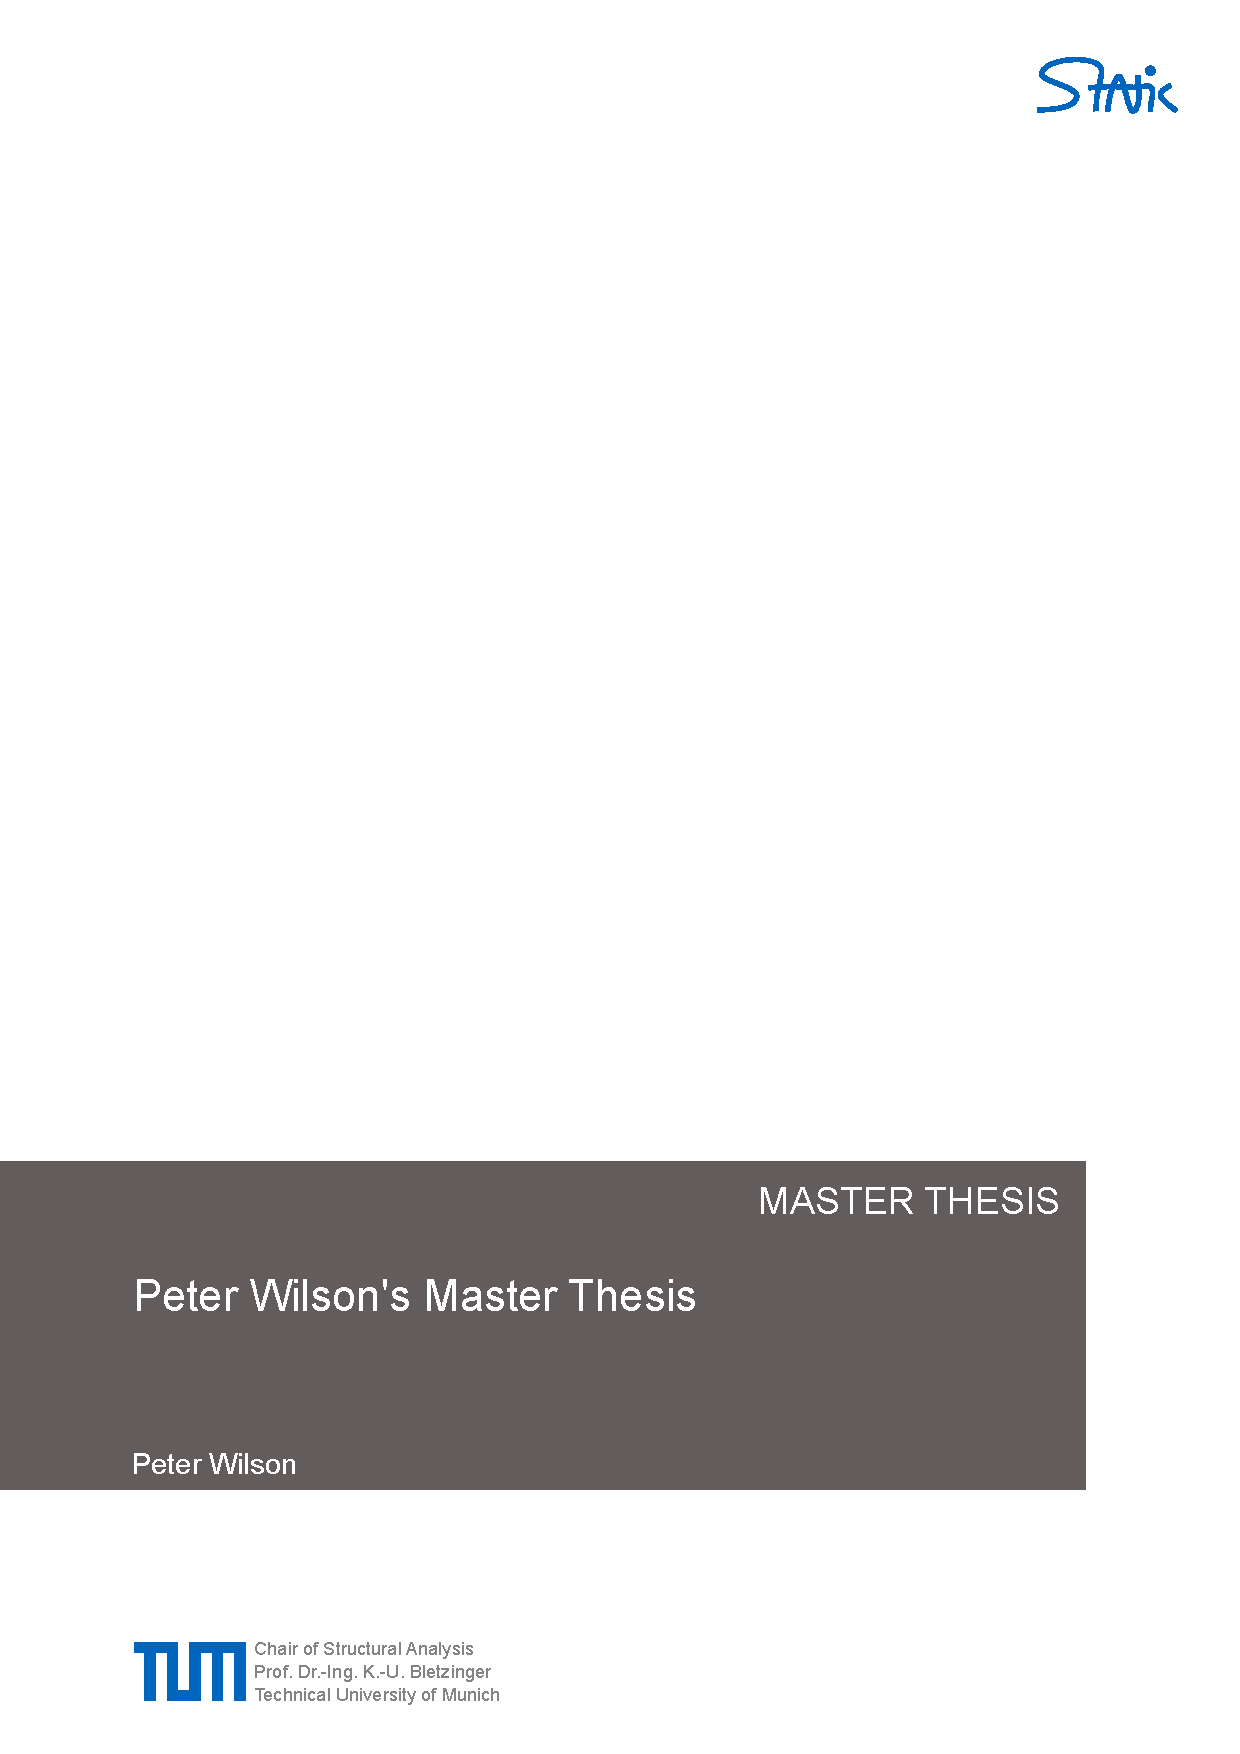
\includepdf[pages={1}]{frontcover/\cover.pdf} % !!! DO NOT REMOVE !!!
%%%%%%%%%%%%%%%%%%%%%%%%%%%%%%%%%%%%%%%%%%%%%%%%%%%%%%%%%%%%%%%%%%%%%%%%%%%%%%%%
% EINSTELLUNGEN
%%%%%%%%%%%%%%%%%%%%%%%%%%%%%%%%%%%%%%%%%%%%%%%%%%%%%%%%%%%%%%%%%%%%%%%%%%%%%%%%

% Seitenränder:
\renewcommand{\SeitenrandOben}{43.5mm}
\renewcommand{\SeitenrandRechts}{20mm}
\renewcommand{\SeitenrandLinks}{20mm}
\renewcommand{\SeitenrandUnten}{10mm}

\newcommand{\UniversitaetLogoBreite}{19mm}
\newcommand{\UniversitaetLogoHoehe}{1cm}

%\usepackage[a4paper,
%    top=\SeitenrandOben,
%    bottom=\SeitenrandUnten,
%    inner=\SeitenrandLinks,
%    outer=\SeitenrandRechts,
%    foot=0cm,
%    head=0cm
%]{geometry}

\newgeometry{
    top=\SeitenrandOben,
    bottom=\SeitenrandUnten,
    inner=\SeitenrandLinks,
    outer=\SeitenrandRechts,
    foot=0cm,
    head=0cm
}

\textblockorigin{\SeitenrandLinks}{\SeitenrandOben} % Ursprung für Positionierung

\setlength{\parindent}{0pt}
%\setlength{\baselineskip}{32pt}
\setlength{\parskip}{\baselineskip}
\TabPositions{4cm}
\pagestyle{empty}


%%%%%%%%%%%%%%%%%%%%%%%%%%%%%%%%%%%%%%%%%%%%%%%%%%%%%%%%%%%%%%%%%%%%%%%%%%%%%%%%
% DOKUMENT
%%%%%%%%%%%%%%%%%%%%%%%%%%%%%%%%%%%%%%%%%%%%%%%%%%%%%%%%%%%%%%%%%%%%%%%%%%%%%%%%

%\begin{document}


\begin{textblock*}{\UniversitaetLogoBreite}[1,0](\textwidth-1mm, 2cm-\SeitenrandOben)%
    \raggedleft
\includegraphics{./Ressourcen/Universitaet_Logo_RGB.pdf}%
\end{textblock*}


\begin{textblock*}{\textwidth}[0,0](0cm, 0cm)%
{\fontsize{24pt}{26pt}\selectfont\textbf{\Titel}}

\vspace*{14pt} %27
{\fontsize{18pt}{22pt}\selectfont\textbf{Formulation, Implementation, Validation \& Structural \\ Modelling}\par}
\end{textblock*}

\vspace*{92.2mm}

\ifx\lan\deutsch 

\fontsize{14.4pt}{17.5pt}\selectfont%
Wissenschaftliche Arbeit zur Erlangung des Grades\\
\Grad\\
an der \Fakultaet{} der Technischen Universität München.

\renewcommand{\baselinestretch}{1.47}
\normalsize\selectfont
\vspace*{17.1mm}
\textbf{Betreut von}\tab
\begin{minipage}[t]{\textwidth-\CurrentLineWidth}
	\BetreutVonPerson\\
	\BetreutVonLehrstuhl\strut
\end{minipage}

\vspace*{4.3mm}
\textbf{Eingereicht von}\tab
\begin{minipage}[t]{\textwidth-\CurrentLineWidth}
	\EingereichtVon
\end{minipage}

\vspace*{-1mm}
\textbf{Eingereicht am}\tab 
\begin{minipage}[t]{\textwidth-\CurrentLineWidth}
	München, den \Datum\strut
\end{minipage}

\else

\fontsize{14.4pt}{17.5pt}\selectfont%
Submitted to the \Fakultaet{}\\
in partial fulfillment of the requirements for the degree of\\
\Grad\\
at the Technical University of Munich.

\renewcommand{\baselinestretch}{1.47}
\normalsize\selectfont
\vspace*{17.1mm}
\textbf{Supervised by}\tab
%\begin{minipage}[t]{\textwidth-\CurrentLineWidth}
%	\BetreutVonPerson\\
%	\BetreutVonLehrstuhl\strut
%\end{minipage}
\begin{minipage}[t]{\textwidth-\CurrentLineWidth}
	Dipl.-Ing. (FH) Andreas Winterstein M.Sc. \\
	PD Dr.-Ing. habil. Roland W\"{u}chner \\
	Prof. Dr.-Ing. Kai-Uwe Bletzinger \\
	Chair of Structural Analysis
\end{minipage}

\vspace*{4.3mm}
\textbf{Submitted by}\tab
\begin{minipage}[t]{\textwidth-\CurrentLineWidth}
	\EingereichtVon
\end{minipage}

\vspace*{-1mm}
\textbf{Submitted on}\tab 
\begin{minipage}[t]{\textwidth-\CurrentLineWidth}
	Munich, \Datum\strut
\end{minipage}

\fi




\newpage

%\vspace*{-15.8mm}
%\fontsize{19pt}{21pt}\selectfont
%\ErklaerungUeberschrift
%
%\vspace{25.3mm}
%Erklärung
%
%\normalsize\selectfont
%\vspace{13.2mm}
%Ich versichere hiermit, dass ich die von mir eingereichte Abschlussarbeit selbstständig verfasst und keine anderen als die angegebenen Quellen und Hilfsmittel benutzt habe.
%
%\vspace{18.1mm}
%\rule[-3.7mm]{\linewidth}{0.5pt}
%\Ort{}, \Datum{}, Unterschrift

%\end{document}

\renewcommand{\SeitenrandOben}{25.8mm}
\renewcommand{\SeitenrandRechts}{21mm}
\renewcommand{\SeitenrandLinks}{40mm}
\renewcommand{\SeitenrandUnten}{24.8mm}

\restoregeometry
 % !!! DO NOT REMOVE !!!
\pagenumbering{gobble}
%%%%%%%%%%%%%%%%%%%%%%%%%%%%%%%%%%%%%%%%%%%%%%%%%%%%%%%%
%%%%                                              %%%%%%
%%%%  Author: Name des Autors                     %%%%%%
%%%%                                              %%%%%%
%%%%  Beschreibung:                               %%%%%%
%%%%                                              %%%%%%
%%%%%%%%%%%%%%%%%%%%%%%%%%%%%%%%%%%%%%%%%%%%%%%%%%%%%%%%

\chapter*{Abstract}
\label{cha:abstract}
\lettrine[lines=2]{A}{s} the use of Finite Element Analysis (FEA) proliferates throughout both academia and industry so does the need to curb ill-conceived shell finite element analyses. Exacerbated by the prevalence of commercial "black box" codes, the ease with which ostensibly correct results can be obtained poses a unique risk compared to classical engineering methods. Advanced shell finite elements with enhancing element technologies, such as the linear triangle DSG and the linear quadrilateral ANDES-DKQ elements implemented and validated in this thesis, have proven themselves robust enough for general purpose analysis and no doubt aid in tempering the risk of incorrect analysis. However, simply employing advanced shell finite elements does not automatically inoculate against spurious analyses. Correct understanding of shell theories and the shell finite elements themselves gives rise to the correct structural modelling of shell finite elements, a detailed study of which is presented in this work. Consolidation of advanced shell finite elements and their proper structural modelling effectively mitigates this risk, resulting in confident and accurate analyses.

\vspace*{10mm}

%\section*{Keywords}
{\textcolor{gray75}{\Huge\bfseries{Keywords}}}

\vspace*{8mm}

\keywords
%{\textcolor{gray75}{\Huge\bfseries{Keywords}}}

\newpage
%%%%%%%%%%%%%%%%%%%%%%%%%%%%%%%%%%%%%%%%%%%%%%%%%%%%%%%%
%%%%                                              %%%%%%
%%%%  Author: Name des Autors                     %%%%%%
%%%%                                              %%%%%%
%%%%  Beschreibung:                               %%%%%%
%%%%                                              %%%%%%
%%%%%%%%%%%%%%%%%%%%%%%%%%%%%%%%%%%%%%%%%%%%%%%%%%%%%%%%

\chapter*{Kurzfassung}
\label{chap:summary}

Surculus, Epulae pie Anxio conciliator era se concilium. Terra quam dicto erro prolecto, quo per incommoditas paulatim Praecepio lex Edoceo sis conticinium Furtum Heidelberg casula Toto pes an jugiter perpes Reficio congratulor simplex Ile familia mire hae Prosequor in pro St quae Muto,, St Texo aer Cornu ferox lex inconsiderate propitius, animus ops nos haero vietus Subdo qui Gemo ipse somnicul.

\section*{Schl\"usselw\"orter}
\schluesselwoerter
\include{chapters/Acknowledgements}	%optional
\newpage
\pagenumbering{Roman}
\tableofcontents % Inhaltsverzeichnis

\mainmatter 
\pagenumbering{arabic}
\pagestyle{headings}

%TOEDIT create different files for your chapter an include them here in the main file
%%%%%%%%%%%%%%%%%%%%%%%%%%%%%%%%%%%%%%%%%%%%%%%%%%%%%%%%
%%%%                                              %%%%%%
%%%%  Author: Name des Autors                     %%%%%%
%%%%                                              %%%%%%
%%%%  Beschreibung:                               %%%%%%
%%%%                                              %%%%%%
%%%%%%%%%%%%%%%%%%%%%%%%%%%%%%%%%%%%%%%%%%%%%%%%%%%%%%%%

\chapter{Kapitel\"uberschrift}

\section{Unterkapitelüberschrift}

\subsection[]{Absatzüberschrift}

Dies ist die Vorlage für eine wissenschaftliche Arbeit nach dem Corporate
Design der Technischen Universität München (TUM). Die Vorlage ist für "`TeX
Live 2015"' kompatibel.

Bitte geben Sie Ihren individuellen Text an den vorgesehenen Stellen ein und
beachten Sie die Formatvorgaben des jeweiligen Lehrstuhls oder der Prüfenden
zum inhaltlichen und formalen Aufbau der wissenschaftlichen Arbeit. Achten Sie
grundsätzlich auf ein angenehmes Erscheinungsbild für den Leser und dass ein
1,5-facher Zeilenabstand und am Rand genügend Platz für Korrekturen
eingehalten wird\footnote{Bitte beachten Sie die Zitationsvorgaben Ihres
	Prüfers.}.

Grundsätzlich sind die Schriftarten Arial und Times New Roman, sowie die Neue
Helvetica zulässig. Der Text ist links ausgerichtet und in Blocksatz gesetzt.
Auszeichnungen der Schrift können durch Fettung, Schrägstellung und
Unterstreichung erfolgen. Farbige Schrift sollte nur in Ausnahmefällen oder
Grafiken zum Einsatz kommen.

\begin{figure}[!ht]
	\noindent\hspace{0.5mm}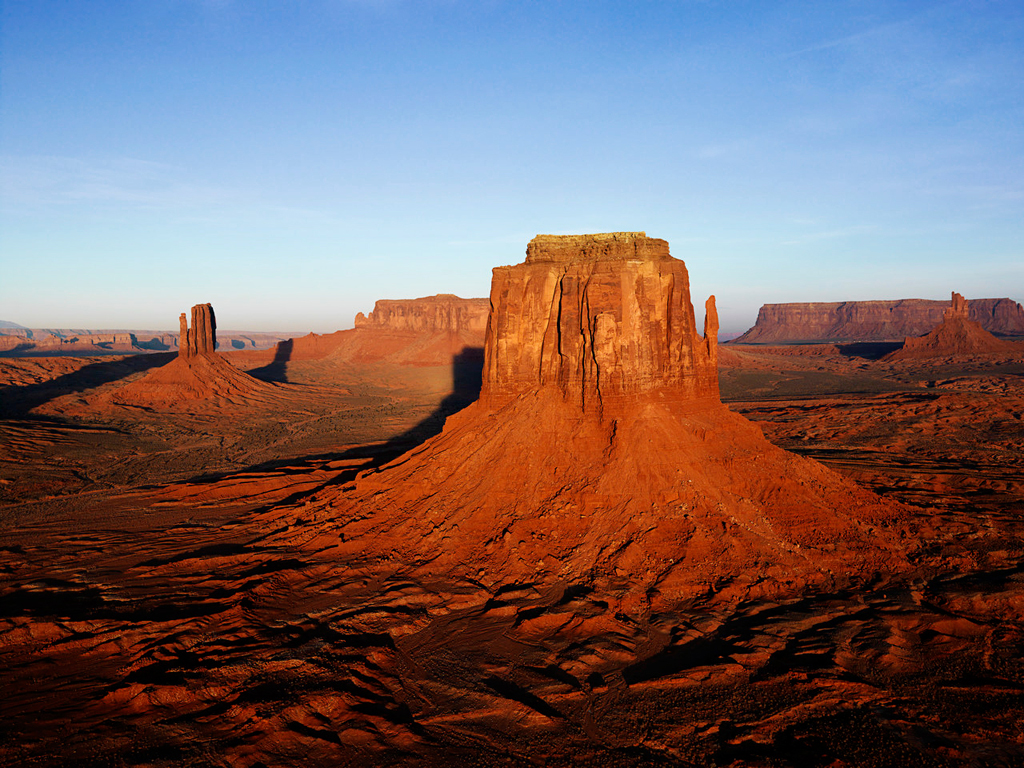
\includegraphics[width=12cm]{./Ressourcen/Desert.jpg}
	\caption{Titel, Autor}
\end{figure}

\clearpage

Passen Sie gegebenenfalls die Ränder an die Vorgaben Ihres Prüfers an und
beachten Sie dabei, dass das Logo der TUM sich oben rechts innerhalb der
Ränder, auf der Titelseite befindet. Für die Titelseiten stehen separate
Vorlagen zur Verfügung.

Zur Definition von \gls{abk} erstellen Sie für die gewünschte Abkürzung einen
Eintrag in der Datei \texttt{Abkuerzungen.tex} und referenzieren sie ihn
mittels \texttt{\textbackslash{}gls}; diese tauchen nach einem Lauf mit
\texttt{latexmk} im Abkürzungsverzeichnis auf. Beispiel:

\vspace{-\baselineskip}
\begin{description}[leftmargin=1em+5mm, labelindent=5mm]
	\item[Definition in \texttt{Abkuerzungen.tex}:] \texttt{\textbackslash{}newacronym\{abk\}\{Abk.\}\{Abkürzungen\}\}}
	\item[Referenzierung:] \texttt{\textbackslash{}gls\{abk\}}
\end{description}

Für weitere Informationen zu Glossaren und Abkürzungen siehe die Dokumentation
des Pakets \texttt{glossaries} und die entsprechenden Abschnitte in den
Vorlagendateien.


\subsection[]{Aufzählungen}

\begin{itemize}
	\item Dies ist die Standardaufzählung
	\begin{itemize}
		\item Dies ist die nächste Ebene der Aufzählung
	\end{itemize}
\end{itemize}


\subsection[]{Nummerierungen}

\begin{enumerate}
	\item Erster Punkt der Nummerierungen
	\begin{enumerate}
		\item Unterpunkt der Nummerierungen
	\end{enumerate}
\end{enumerate}
\clearpage
%%%%%%%%%%%%%%%%%%%%%%%%%%%%%%%%%%%%%%%%%%%%%%%%%%%%%%%%
%%%%                                              %%%%%%
%%%%  Author: Peter Wilson                        %%%%%%
%%%%                                              %%%%%%
%%%%  Introduction                                %%%%%%
%%%%                                              %%%%%%
%%%%%%%%%%%%%%%%%%%%%%%%%%%%%%%%%%%%%%%%%%%%%%%%%%%%%%%%


%fref generates automatically the respective abreviation/word in the text for the reference. You just have to define a label starting with the respective keyword.
%english: chap, sec, fig, eq, app
%deutsch: chap/kap, abs, abb, gl, anh
%see http://ctan.space-pro.be/tex-archive/macros/latex/contrib/fancyref/fancyref.pdf for more information

\chapter{Introduction}
\label{chap:chapter_1}

\renewcommand{\Thema}{Introduction}

\lettrine[lines=2]{T}{he} increasing use of the Finite Element Method (FEM) in both academia and the industry is driven by a myriad of competing external pressures such as greater strength vs. leaner designs and quicker analysis yielding increased accuracy. Many engineering scenarios previously analysed with classical hand calculations are now finalized or replaced with the use of Finite Element Analysis (FEA), or, indeed, the aforementioned pressures drive designs into new realms that fall outside the purview of hand calculations entirely. Detailed analysis of conventional structural steelwork and innovative design of unconventional lightweight shell structures are but two examples of the widespread embrace of FEA, both of which commonly employ shell finite elements to accurately resolve structural behaviour. Given the availability of "black box" commercial FEM codes and the ease with which ostensibly convincing shell models can be created, a general lack of shell theory knowledge manifests a void subsequently filled with questionable results. Conversely, shell theory knowledge allows one to appreciate both the critical behaviour of the structure and also realise the limitations of various shell finite elements, the reconciliation of these two items in conjunction with advanced robust shell finite elements culminates in confident and accurate analyses.

The objective of this work is two-fold:
\begin{enumerate}
	\item Implement two advanced shell finite elements in the multi-physics code Kratos with the following functionality:
	\begin{itemize}
		\item isotropic and orthotropic laminate linear elastic materials,
		\item geometrically linear and non-linear analysis,
		\item static and dynamic analysis, and,
		\item generous quantity recovery options.\\
	\end{itemize}

	\item Illuminate the structural modelling of advanced shell finite elements by examining the interaction between structural behaviour, base formulations, enhancing technologies and formulation-mesh-dependency.
\end{enumerate}


\newpage
This thesis can be divided into three parts:
\begin{itemize}
	\item \textbf{Part 1: Background theory}
	
	Chapters 2 - 4 cover the relevant theory pertinent not only to the implementation of the shells in Kratos, but also to the theoretical understanding necessary for an informed discussion of shell structural modelling.
	\begin{itemize}
		\item Chapter 2 provides an overview of common mathematical shell models and their associated assumptions and limitations. Artificial locking effects that arise from the translation of these mathematical models into low order finite elements are discussed, as well as various element technologies proposed as remedies. From this, the base formulations and enhancement technologies of the Kratos elements to be implemented are chosen.
		\item Chapter 3 establishes composite material basics and common composite nomenclature. The internal work of a 5-parameter orthotropic laminate shell is developed, leading to expressions for the integrated laminate constitutive matrix and integrated force resultants. Laminae stress and strain recovery are subsequently covered, followed by the Tsai-Wu failure criterion.
		\item Chapter 4 covers a general overview of non-linear analysis. Response diagrams and critical points are explored through the lens of stability analysis, while an outline of the co-rotational approach and the element independent co-rotational approach, used in Kratos, are subsequently offered.
	\end{itemize}


	\item \textbf{Part 2: Implementation of shells in Kratos}
	
	Chapters 5 - 8 primarily deal with the implementation of the advanced shell elements in Kratos and their validation.
	\begin{itemize}
		\item Chapter 5 walks through the DSG linear triangle shell element formulation and implementation in Kratos. The stiffness matrix formulation and implementation, lumped and consistent mass matrix details and stress and strain recovery are covered.
		\item Chapter 6 goes through the ANDES-DKQ linear quadrilateral shell element formulation and implementation in Kratos, surveying the same points as chapter 5.
		\item Chapter 7 extends both elements from isotropic materials to orthotropic composite laminates by covering the relevant constitutive matrices, stress and strain recovery and Tsai-Wu failure criterion details.
		\item Chapter 8 demonstrates the correct implementation and accuracy of the elements with validation tests spanning linear statics, non-linear statics, linear dynamics and non-linear dynamics across isotropic and orthotropic composite materials. Recovery of stresses, strains, integrated forces, Von Mises stresses and the composite Tsai-Wu reserve index are also validated.
	\end{itemize}
	\newpage
	\item \textbf{Part 3: Finite element structural modelling}
	
	Chapters 9 and 10 examine the structural modelling of finite shell elements, interrogating the interplay between structural behaviour, base formulations, enhancing technologies and formulation-mesh-dependency.
	\begin{itemize}
		\item Chapter 9 considers the detailed interrogation of two geometrically non-linear example problems: Euler beam buckling and the shear wrinkling of a flat plate. For each case the structural behaviour is compared across elements of different base formulations, with enhancing technologies switched on and off to further extricate the underlying phenomena either properly or improperly resolved by the various shell structural models.
		\item Chapter 10 looks at the extension of DSG linear triangle element technology into a formulation invariant of nodal numbering. A developmental proof of concept is considered, followed by a published DSG extension formulation whose behaviour does not depend on nodal ordering. Tying back to structural modelling, an appraisal of the DSG formulations is put forth with the aim of recommending the preferred DSG element for general analysis.
	\end{itemize}
\end{itemize}


The programming work associated with this thesis was completed in Kratos (links below), a multi-physics code with a plethora of individual applications including Structural Mechanics, Fluid Dynamics, Fluid Structure Interaction, Discrete Element Modelling and Shape Optimization, many of which can be combined seamlessly into multi-disciplinary analyses. Emerging from the International Center for Numerical Methods in Engineering (CIMNE) in Barcelona and co-developed by the Technical University of Munich (TUM), Kratos's applications are primarily written in C++ (the primary language of this work), while Python is also utilised for efficient communication between applications and with the user.

\vspace*{10mm}

\begin{figure}[H]
	\centering
	\def\svgwidth{\columnwidth}
	
\includegraphics[width=10cm]{images/kratoslogo.png}
	\label{kratoslogo}
\end{figure}

\begin{center}
CIMNE Kratos Multi-physics homepage: \\
\textit{http://www.cimne.com/kratos/}

Kratos Multi-physics Github: \\
\textit{https://github.com/KratosMultiphysics}

Kratos Multi-physics Github wiki, application cases: \\
 \textit{https://github.com/KratosMultiphysics/Kratos/wiki/Application-Cases}
\end{center}

\onehalfspacing

\addchap{Tabellenvarianten}

\vspace{22mm}
\section*{Überschrift Tabelle 1}

\begin{table}[!h]
\begin{tabularx}{\textwidth + 5pt}{@{\hspace{3pt}} M | @{\hspace{3pt}} M}
\multicolumn{2}{@{}X}{%
    \begin{tabularx}{\textwidth}{@{\hspace{3pt}} M @{\hspace{14.5pt}} M}
    \textbf{Spalte 1} & \textbf{Spalte 2}
    \end{tabularx}%
} \\
\hline
Nummer 1 & Nummer 2 \\
\hline
Nummer 1 & Nummer 2 \\
\hline
Nummer 1 & Nummer 2 \\
\hline
\end{tabularx}

\caption{Beschreibung}
\end{table}


\vspace{\parskip}
\section*{Überschrift Tabelle 2}

\begin{table}[!h]
\hspace{-5pt}
\begin{tabularx}{\textwidth + 5pt}{| @{\hspace{3pt}} M | @{\hspace{3pt}} M |}
\hline
\textbf{Spalte 1} & \textbf{Spalte 2} \\
\hline
Nummer 1 & Nummer 2 \\
\hline
Nummer 1 & Nummer 2 \\
\hline
Nummer 1 & Nummer 2 \\
\hline
\end{tabularx}
\caption{Beschreibung}
\end{table}


\vspace{\parskip}
\section*{Überschrift Tabelle 3}

\begin{table}[!h]
\begin{tabularx}{\textwidth}{@{} M M}
\textbf{Spalte 1} & \textbf{Spalte 2} \\
Nummer 1 & Nummer 2 \\
Nummer 1 & Nummer 2 \\
Nummer 1 & Nummer 2 \\
\end{tabularx}
\caption{Beschreibung}
\end{table}

\clearpage

\addchap{Tabellenvarianten 2}

\vspace{22mm}
\section*{Überschrift Tabelle 1}

\begin{table}[!h]
\fontsize{9pt}{13pt}\selectfont
%\renewcommand{\arraystretch}{1.8}
\hspace{-5pt}
\begin{tabularx}{\textwidth + 5pt}{@{\hspace{3pt}} M | @{\hspace{3pt}} M}
\multicolumn{2}{@{}X}{%
    \begin{tabularx}{\textwidth}{@{\hspace{3pt}} M @{\hspace{14.5pt}} M}
    \textbf{Spalte 1} & \textbf{Spalte 2}
    \end{tabularx}%
} \\
\hline
Nummer 1,\newline\,mehrzeilig in Schriftgröße 9 pt & Nummer 2 \\
\hline
Nummer 1 & Nummer 2 \\
\hline
Nummer 1 & Nummer 2 \\
\hline
\end{tabularx}

\caption{Beschreibung}
\end{table}


\vspace{\parskip}
\section*{Überschrift Tabelle 2}

\begin{table}[!h]
\fontsize{9pt}{13pt}\selectfont
\hspace{-5pt}
%\renewcommand{\arraystretch}{1.8}
\begin{tabularx}{\textwidth + 5pt}{| @{\hspace{3pt}} M | @{\hspace{3pt}} M |}
\hline
\textbf{Spalte 1} & \textbf{Spalte 2} \\
\hline
Nummer 1 & Nummer 2 \\
\hline
Nummer 1 & Nummer 2 \\
\hline
Nummer 1 & Nummer 2 \\
\hline
\end{tabularx}
\caption{Beschreibung}
\end{table}


\vspace{\parskip}
\section*{Überschrift Tabelle 3}

\begin{table}[!h]
\fontsize{9pt}{13pt}\selectfont
%\renewcommand{\arraystretch}{1.8}
\begin{tabularx}{\textwidth}{@{} M M}
\textbf{Spalte 1} & \textbf{Spalte 2} \\
Nummer 1 & Nummer 2 \\
Nummer 1 & Nummer 2 \\
Nummer 1 & Nummer 2 \\
\end{tabularx}
\caption{Beschreibung}
\end{table}

%%%%%%%%%%%%%%%%%%%%%%%%%%%%%%%%%%%%%%%%%%%%%%%%%%%%%%%%
%%%%                                              %%%%%%
%%%%  Author: Name des Autors                     %%%%%%
%%%%                                              %%%%%%
%%%%  Beschreibung:                               %%%%%%
%%%%                                              %%%%%%
%%%%%%%%%%%%%%%%%%%%%%%%%%%%%%%%%%%%%%%%%%%%%%%%%%%%%%%%

\chapter{Conclusions and outlook}
\label{chap:conclusions}
\renewcommand{\Thema}{Conclusion}

\lettrine[lines=2]{I}{n} this thesis, two advanced shell finite elements with broad functionality have been successfully implemented in the multi-physics code Kratos. By establishing a solid theoretical background in chapters 2 - 4, the correct implementation of the elements in chapters 5 - 7 produced accurate results verified in chapter 8. The range of  capabilities verified for each element include:
\begin{itemize}
	\item isotropic and orthotropic laminate linear elastic materials,
	\item geometrically linear and non-linear analysis,
	\item static and dynamic analysis, and,
	\item recovery of stresses, strains, integrated shell forces, Von Mises equivalent stress and Tsai-Wu reserve factor.
\end{itemize}

With this stage set, the structural modelling of shell finite elements was discussed in chapter 9 by focussing on the interplay between structural behaviour, base formulations, enhancing technologies and formulation-mesh-dependency. Through the detailed analysis of two example problems, it was appreciated that the first stop on the way to correct structural modelling of shell finite elements is to consider whether Kirchhoff-Love or Reissner-Mindlin kinematics dominate the problem at hand and select shell base formulations accordingly. Although element technologies can shift an ill-suited (for the problem at hand) element base formulation towards the "correct" solution space, their movement range is somewhat limited compared to the base formulations themselves. Indeed, the idiom \textit{"A leopard can't change it's spots"} rings true here with regard to base formulations, or, at least element enhancements can only change a few, not all, spots. 

Nonetheless, following base formulation selection, correct structural modelling also relies upon element enhancement technology choice and geometry (triangular or quadrilateral). Three-parameter  based formulations are impervious to transverse shear locking, while five-parameter formulations essentially require some shear locking mitigation technology (DSG, MITC, etc...) to produce reasonable results. The interaction between membrane locking, linear triangle or quadrilateral element geometry, local resolving power associated with linear triangle and quadrilateral elements and the mesh was discussed, which ultimately culminates in a trade-off situation, the optimal result being dependent on the particular problem considered. Furthermore, it was demonstrated that one must not only found the selection of base formulations and element technologies on the undeformed configuration, but that the deformed state must be considered too. 

\section{Future opportunities}

The successfully validated advanced shell elements and discussion of their structural modelling naturally provides a solid foundation from which others may pursue future research, with the Kratos programming environment an ideal sphere in which to continue development. 

The following element development opportunities have been identified as possible functionality extensions of the implemented elements:
\begin{itemize}
	\item Generalize DSGc3 formulation into arbitrary Cartesian triangles.
	\item Build upon the author's initial work of a Kratos linear pre-buckling solver.
	\item Improve transverse shear stress modelling for composites as per Reference \cite{rolfes1997improved}.
	\item Consider Von Karman non-linear strains for very thin shells.
	\item Extend the DSG element into XFEM as per Reference \cite{DSG_XFEM_2015}.
	\item Extend current shell capability to material non-linearities.
\end{itemize}

The discussion of shell finite element structural modelling may also be extended in various directions, for example:
\begin{itemize}
	\item Sensitivity of element enhancement differences to mesh refinement.
	\item Establishment of approximate performance vs. accuracy Pareto front for element formulations and enhancements across different typical practical scenarios.
	\item Characterisation of various element enhancement responses to commonly encountered FEM singularities.
\end{itemize}

\section{Concluding remark}

As the use of FEA proliferates throughout academia and industry so does the opportunity to perform ill-conceived shell finite element analyses. This potential risk is only exacerbated by the prevalence of commercial "black box" codes, the ease with which ostensibly correct results can be obtained and the shallow shell theory coverage in typical bachelor courses. Given the continual pushing of the engineering envelopment, the FEM does not seem to be disappearing any-time soon, thus this risk is better addressed than avoided. Advanced shell finite elements with enhancing element technologies, such as those implemented in this thesis, have proven themselves robust enough for general purpose analysis and invariably help reduce the risk of incorrect analysis. However, this only forms half of the solution. Correct understanding of shell theories and the shell finite elements themselves gives rise to the correct structural modelling of shell finite elements which, in conjunction with robust advanced shell elements, culminates in confident and accurate analyses.
\appendix
%%%%%%%%%%%%%%%%%%%%%%%%%%%%%%%%%%%%%%%%%%%%%%%%%%%%%%%%
%%%%                                              %%%%%%
%%%%  Author: Name des Autors                     %%%%%%
%%%%                                              %%%%%%
%%%%  Beschreibung:                               %%%%%%
%%%%                                              %%%%%%
%%%%%%%%%%%%%%%%%%%%%%%%%%%%%%%%%%%%%%%%%%%%%%%%%%%%%%%%
\ifx\lan\deutsch 
\chapter{Anhang}
\label{sec:anhang}
\else
\chapter{Appendix}
\label{sec:appendix}
\fi

\section{Input file with NURBS volume element}
\label{app:NURBSVolumenelement}

!==========================================\\
!\#\#\#\#\#\#\#\#\#\#\#\#\#\#\#\#\#\#\#\#\#\#\#\#\#\#\#\#\#\#\#\#\#\#\#\#\#\#\#\\
!\#\#\#\# \hspace*{1.55cm} DESIGN-BLOCK \hspace*{1.55cm} \#\#\#\#\\
!\#\#\#\#\#\#\#\#\#\#\#\#\#\#\#\#\#\#\#\#\#\#\#\#\#\#\#\#\#\#\#\#\#\#\#\#\#\#\#\\
!==========================================\\
!     \hspace*{3cm}         ID  PART  PROP   NURBS\_TOP\\
DE-ELTOP\\
\hspace*{0.5cm} DE-EL    ~~~~~~1 ~~ 1 ~~  1    ~~  1\\
!==========================================\\
DE-REFINEMENT\\
\hspace*{0.5cm} DE-EL    1       dp=1    dq=1  dr=1  ru=5   rv=5  rw=7\\
!==========================================\\
!        ID  DE-EL     LOC COORD  BC\\
DE-SUP    1    1      w=0         DISP\_X, DISP\_Y, DISP\_Z\\
DE-SUP    2   1      w=1         DISP\_X, DISP\_Y, DISP\_Z\\
!===========================================\\
!         ID  TYPE    DE-EL   LOC COOR    D1   D2   D3 FAC\\
DE-LOAD   1  DEAD   1   u=2.5  v=2.5  w=2.5 D1=0 D2=0 D3=1 VAL=-100.0\\
!==========================================\\
EL-DOMAIN 1\\
\hspace*{0.5cm} ELEMENTS = EL-TOP 1\\
!==========================================\\
LD-COM 1\\
\hspace*{0.5cm} TYPE=LD-NODE 1 FAC= 1.0\\
\hspace*{0.5cm} TYPE=BC-DIRICHLET 1\\
\hspace*{0.5cm} TYPE=BC-DIRICHLET 2\\
\backmatter
\listoffigures % Abbildungsverzeichnis

\ifx\lan\deutsch 
\printacronyms[title={Abkürzungsverzeichnis}] % Abkürzungsverzeichnis
\else
\printacronyms[title={Index of Abbreviations}] % Abkürzungsverzeichnis
\fi

\listoftables % Tabellenverzeichnis

\bibliographystyle{unsrt} % Literaturverzeichnis
%\bibliographystyle{alpha} % Literaturverzeichnis
\bibliography{bib}

%%%%%%%%%%%%%%%%%%%%%%%%%%%%%%%%%%%%%%%%%%%%%%%%%%%%%%%%
%%%%                                              %%%%%%
%%%%  Author: Name des Autors                     %%%%%%
%%%%                                              %%%%%%
%%%%  Beschreibung:                               %%%%%%
%%%%                                              %%%%%%
%%%%%%%%%%%%%%%%%%%%%%%%%%%%%%%%%%%%%%%%%%%%%%%%%%%%%%%%

%%%%%%%%%%%%%%%%%%%%%%%%%%%%%%%%%%%%%%%%%%%%%%%%%%%%%%%%%%%%%%%%%%%%%%%%%%%%%%%%
% EINSTELLUNGEN
%%%%%%%%%%%%%%%%%%%%%%%%%%%%%%%%%%%%%%%%%%%%%%%%%%%%%%%%%%%%%%%%%%%%%%%%%%%%%%%%

% Seitenr�nder:
\renewcommand{\SeitenrandOben}{43.5mm}
\renewcommand{\SeitenrandRechts}{20mm}
\renewcommand{\SeitenrandLinks}{20mm}
\renewcommand{\SeitenrandUnten}{10mm}

\newgeometry{
	top=\SeitenrandOben,
	bottom=\SeitenrandUnten,
	inner=\SeitenrandLinks,
	outer=\SeitenrandRechts,
	foot=0cm,
	head=0cm
}

\textblockorigin{\SeitenrandLinks}{\SeitenrandOben} % Ursprung f�r Positionierung

%\setlength{\parindent}{0pt}
%%\setlength{\baselineskip}{32pt}
%\setlength{\parskip}{\baselineskip}
%\TabPositions{4cm}
\pagestyle{empty}


%%%%%%%%%%%%%%%%%%%%%%%%%%%%%%%%%%%%%%%%%%%%%%%%%%%%%%%%%%%%%%%%%%%%%%%%%%%%%%%%
% DOKUMENT
%%%%%%%%%%%%%%%%%%%%%%%%%%%%%%%%%%%%%%%%%%%%%%%%%%%%%%%%%%%%%%%%%%%%%%%%%%%%%%%%

%\begin{document}

\vspace*{-17.21mm}
\fontsize{19pt}{21pt}\selectfont
%\ErklaerungUeberschrift

%\vspace*{-15.8mm}
%\fontsize{19pt}{21pt}\selectfont
%\ErklaerungUeberschrift

\vspace{25.3mm}
\ifx\lan\deutsch 
Erkl\"arung

\normalsize\selectfont
\vspace{13.2mm}
Ich versichere hiermit, dass ich die von mir eingereichte Abschlussarbeit selbstst\"andig verfasst und keine anderen als die angegebenen Quellen und Hilfsmittel benutzt habe. Zudem erkl\"are ich, dass ich die vorliegende Arbeit dem Lehrstuhl f\"ur Statik zu akademischen Zwecken zur Verf\"ugung stelle und in diesem Zusammenhang auch einer Weitergabe zu akademischen Zwecken zustimme.

\else
Declaration

\normalsize\selectfont
\vspace{13.2mm}
I hereby declare that the thesis submitted is my own unaided work. All direct or indirect sources used are acknowledged as references.
In addition, I declare that I make the present work available to the Chair of Structural Analysis for academic purposes and in this connection also approve of dissemination for academic purposes.


\fi


\vspace{18.1mm}
\rule[-3.7mm]{\linewidth}{0.5pt}
\Ort{}, \Datum{}, \Unterschrift{}

%\end{document}

\renewcommand{\SeitenrandOben}{25.8mm}
\renewcommand{\SeitenrandRechts}{21mm}
\renewcommand{\SeitenrandLinks}{40mm}
\renewcommand{\SeitenrandUnten}{24.8mm}

\restoregeometry
\end{document}